\documentclass{book}
\usepackage{textcomp}
\usepackage{hyperref}
\usepackage{graphicx}
\usepackage{ifthen}
\usepackage{multicol}
\usepackage{makeidx}

\makeindex

\newcommand{\half}{$\frac{1}{2}$}
\newcommand{\quarter}{$\frac{1}{4}$}
\newcommand{\threequarter}{$\frac{3}{4}$}
\newcommand{\eighth}{$\frac{1}{8}$}
\newcommand{\third}{$\frac{1}{3}$}
\newcommand{\twothird}{$\frac{2}{3}$}
\newcommand{\Tp}[1]{#1\,tbsp}
\newcommand{\tp}[1]{#1\,tsp}
\newcommand{\C}[1]{#1\,cup}
\newcommand{\oz}[1]{#1\,oz}
\newcommand{\cm}[1]{#1\,cm}
\newcommand{\inch}[1]{#1$^{\prime\prime}$}
\newcommand{\lbs}[1]{#1\,lbs}
\newcommand{\qt}[1]{#1\,qt}
\newcommand{\gr}[1]{#1\,g}
\newcommand{\kgr}[1]{#1\,kg}
\newcommand{\gal}[1]{#1\,gallon}
\newcommand{\ltr}[1]{#1\,L}
\newcommand{\mL}[1]{#1\,mL}
\newcommand{\tF}[1]{#1\,\textdegree F}
\newcommand{\tC}[1]{#1\,\textdegree C}
\newcommand{\ang}[1]{#1\,\textdegree}
\newcommand{\UNTESTED}{ $\bullet$ }
\newcommand{\FIXME}{ $\star$ }

\newenvironment{ingredients}
{\noindent\textit{Ingredients:}\renewcommand{\item}{\par\noindent}}{\par}

\newenvironment{directions}
{\smallskip\begin{enumerate}\setlength{\itemsep}{-1pt}}{\end{enumerate}}

\catcode`\@=11
%    \@car is actually already defined in latex.tex, but for
%    maximum robustness it needs to have the \long prefix:
\long\def\@car#1#2\@nil{#1}
\long\def\@first#1#2{#1}
\long\def\@second#1#2{#2}
\long\def\ifempty#1{\expandafter\ifx\@car#1@\@nil @\@empty
  \expandafter\@first\else\expandafter\@second\fi}
  \catcode`\@=12
  
  \long\def\test#1{\begingroup \toks0{[#1]}%
    \newlinechar`\/\message{/\the\toks0:
      \ifempty{#1}{EMPTY}{NOT empty}%
      }\endgroup}
      
\newcommand{\nonempty}[2]{\ifempty{#1}{}{#2}}

\newenvironment{recipe}[3]{

\newcommand{\theme}[1]{\index{##1!#1}##1}

\section{#1}
\nonempty{#2#3}{
\noindent
	\nonempty{#2}{From #2.}
\hfil 
	\nonempty{#3}{Makes #3.}
\par}
\begin{multicols}{2}
}{\end{multicols}}

\newcommand{\hint}[1]{\smallskip \noindent \textsl{#1} \par}
\newcommand{\subrecipe}[1]{\subsection*{#1}}


\begin{document}

\title{Laboratory Procedures for Basic Applied Biochemistry \\
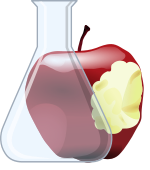
\includegraphics[width=10cm]{CoverLogo} 
}
\author{ Andre Masella }
\date{\today{} -- \input{Revision.tex}}
\maketitle

\tableofcontents

\chapter{ Introduction }

\section { Welcome }

These are recipes I have collected from various places. Most of them are
family recipies. Some recpies are marked \UNTESTED meaning I have not
made them, but they seem sound.  I will test them eventually.\par

\section { Preparation }

This has been typeset using \LaTeX{}, using custom recipe environments.
The cover graphic was made in Kontour.\par

\section { Conversion Hints }

Baking is mostly imperial, but I am a very metric person. Since a cup is
125\,mL which is realtively ``round'' number, I can live with the
inconsitancies, but it is good to know that: \par

\begin{tabular}{c c c c c}
3 tsp & = & 1 tbsp & = & \half oz \\
1 cup & = & 8 oz & = & \quarter qt 
\end{tabular}

\section { Bread Cooking }
According to Alton Brown, bread should be cooked until it reaches an internal termperature of \tF{207}. Any higher than \tF{210} or lower than \tF{205} will result in bad bread. Times are suggestions based on experience before cooking by temperature or for recipes where inserting a temperature probe is not practical. Any recipes where bread is not cooked to \tF{207} are explicitly labelled.

\chapter{Pasta Sauce}
\begin{recipe}{Pasta Romana}{Franco Iori}{}

\begin{ingredients}
\item 1~clove of garlic, halved
\item \gr{225} spaghetti or linguine
\item one large handful of chopped parsley
\item \C{\half} of white wine
\item olive oil
\item salt
\item \htheme{Parmesan}{cheese}, grated
\end{ingredients}

\begin{directions}
\item Bring a pot of salted water to a boil. Once boiling, add the pasta.
\item Sweat garlic in olive oil.
\item Remove from the heat and allow to cool slightly (to prevent a fireball in the next stage).
\item Add the parsley and white wine.
\item Put back on heat and cook until the pasta is approximately 1~minute from being done.
\item Drain pasta, leaving some water behind, and return to pot.
\item Add contents of frying pan to pot and cook for remaining minute.
\item Add cheese and serve immediately.
\end{directions}

\hint{You can also add a combination of sliced black olives or anchovies when adding the parsley.}
\end{recipe}



\printindex

\end{document}
